
\documentclass[11pt,a4paper]{article}
\usepackage[left=2cm,right=2cm,top=2cm,bottom=3cm]{geometry}
\usepackage{amsmath,amsfonts,amsthm,amssymb,varioref,times, commath}
\usepackage{gensymb}
\usepackage{tikz}
\usepackage{textcomp}
\usepackage{hyperref}
\hypersetup{
 colorlinks=true,
 linkcolor=blue,
 filecolor=magenta, 
urlcolor=cyan,
}
\usepackage{lipsum}
\usepackage{epigraph}
%to resume numbering in a list
\usepackage{enumitem}
%----- arrows 
\usepackage{extarrows}

%    differential equatiosn 
\usepackage{diffcoeff}   %\diff[2]{x}{y}


%%%%%%pour ecrire en français avec les accents
\usepackage[utf8]{inputenc}
\usepackage[T1]{fontenc}
\usepackage{lmodern} % load a font with all the characters
\usepackage{units}
%%%%%%%Image-related packages
\usepackage{wrapfig}
\usepackage{float, graphicx}
\graphicspath{ {./img/} }
\usepackage{subcaption}
\usepackage[export]{adjustbox}

%%%%%%%pour faire des cadres
\usepackage{xcolor}
\usepackage{tcolorbox}
\usepackage{framed}
\usepackage{mdframed}


%%%%%%%chemistry frmulae
\usepackage{chemfig}
\usepackage{chemformula}
\usepackage[version=4]{mhchem}

% -------------- Circuits -------------------
\usepackage[european, straightvoltages]{circuitikz}

% Title & headers
\usepackage[explicit]{titlesec}
% Raised Rule Command:
% Arg 1 (Optional) - How high to raise the rule
% Arg 2 - Thickness of the rule
\newcommand{\raisedrulefill}[2][0ex]{\leaders\hbox{\rule[#1]{1pt}{#2}}\hfill}
\titleformat{\section}{\Large\bfseries}{\thesection. }{0em}{#1\,\raisedrulefill[0.4ex]{1pt}}

% pour ecrire sur +sieurs colonnes
\usepackage{multicol}
\setlength{\columnseprule}{0pt}
\setlength{\columnsep}{60pt}
% Fusion de lignes de tableaux.
\usepackage{multirow}
% Position verticale des lettres dans la ligne de tableau.
\usepackage{array}

% physics -----------------------------------------------------------
\newcommand{\To}{\longrightarrow}
\newcommand{\gpl}{\; g\cdot L^{-1}}
\newcommand{\gpmol}{\; g\cdot mol^{-1}}
\newcommand{\mpl}{\; mol\cdot L^{-1}}
\newcommand{\mps}{\; m\cdot s^{-1}}
\newcommand{\rps}{\; rad\cdot s^{-1}}
\newcommand{\kph}{\; km\cdot h^{-1}}
\newcommand{\mpss}{\; m\cdot s^{-2}}
\newcommand{\Dt}{\Delta t}
\newcommand{\vv}{\vec{v}}
\newcommand{\va}{\vec{a}}
\newcommand{\vp}{\vec{p}}
\newcommand{\vf}{\vec{F}}
\newcommand*{\Vf}[1]{\overrightarrow{F_\ensuremath{{#1}}}}
\newcommand{\es}[1]{\cdot10^{#1}}
\newcommand{\eng}[1]{\textcolor{purple}{(= #1})}
\usepackage{harpoon}
%\newcommand*{\vect}[1]{\overrightharp{\ensuremath{#1}}}
\newcommand*{\Vect}[1]{\overrightarrow{\ensuremath{#1}}}
\newcommand{\pfd}[1]{\sum \vec{F}_{ext_{#1}} &= \od{\vp_{#1}}{t} = m\cdot\va_{#1}}
\newcommand{\C}{\degree C}
\newcommand{\Delt}{\Delta t}

% --- Circuits ------------
\newcommand{\bipole}[1]{
\begin{circuitikz} \draw
(0,0) to[ #1 ] (2,0); 
\end{circuitikz} {\hspace{5mm}}}

% Chimie ---------------------------------
\newcommand{\oxo}{\ce{H3O+}_{(aq)}}
\newcommand{\eau}{\ce{H2O}_{(\ell)}}
\newcommand{\OH}{\ce{HO-}_{(aq)}}
\newcommand{\AH}{\ce{AH}_{(aq)}}
\newcommand{\A}{\ce{A-}_{(aq)}}
\newcommand{\MnO}{\ce{MnO_4^{-}}}
\newcommand{\conc}[1]{\left[{#1}\right]}
\newcommand{\couple}[2]{\ce{#1/#2}}


% Environnements ------------------------
\newcounter{exo}
\newenvironment{exo}[1][]
{\refstepcounter{exo} \begin{shaded}\noindent $\triangleright \quad$\textbf{Exercice~\theexo. #1} } { \end{shaded}}
\newenvironment{eg}
{\begin{shaded} \textbf{Exemple:} } { \end{shaded}}

\newenvironment{defn}[1]
{\begin{leftbar}\noindent \textbf{Définition :\textit{ \quad #1}} } { \end{leftbar}}

%\newenvironment{rmrq}
%{\begin{shaded} \textbf{Remarque.\quad } \itshape } { \end{shaded}}
\newenvironment{rmrq}
{\begin{mdframed}[backgroundcolor=blue!10, linewidth=0pt] \textbf{Remarque.\quad } \itshape } { \end{mdframed}}

\newenvironment{python}
{\begin{shaded} \textbf{A faire en PYTHON}\\ \itshape } { \end{shaded}}

% Shading colour -----------------------------
\definecolor{shadecolor}{gray}{0.9}

\date{}
\author{}

\renewcommand*\contentsname{Résumé}









% Title & headers 
\usepackage{fancyhdr}
\pagestyle{fancy}
\fancyhf{}
\lhead{SciPhy : Terminale spé}
\rhead{$\Phi$ - 5 : Ondes}
\chead{2020-28}
\rfoot{Page \thepage}
\lfoot{\textcopyright\; S Zayyani}
\renewcommand{\footrulewidth}{0.1pt}% default is 0pt

\title{\large Physique - Chapitre 5 \\ \LARGE Phénomènes Ondulatoires}
\date{}
\author{}

\setlength{\parindent}{0mm}
\setlength{\parskip}{2mm}

%%%%%%%%%%% For wrapfigure 
\setlength{\intextsep}{6pt}%
\setlength{\columnsep}{3pt}%



\begin{document}
\maketitle
\vspace{-1cm}
\begin{tcolorbox}[title=Notions de la classe de première à rappeler]
Ondes ; caractéristiques des ondes 
%\tcblower
\end{tcolorbox}
\tableofcontents
\newpage

\section{Rappels : Ondes}
Avant de parler de ce qu'est un son, revenons à la définition d'une onde. 

\begin{defn}{Ondes}
\begin{itemize}
    \item Une perturbation \eng{disturbance} est une modification locale  et temporaire des propriétés physiques d'un milieu (e.g. la déformation dans une corde, la déformation de la surface d'eau).
    \item On appelle \textbf{onde mécanique} le phénomène de propagation d'une perturbation dans un milieu matériel, \textbf{sans transport de matière}.
    \item Une onde est une onde progressive si la perturbation se propage dans le milieu (nous verrons plus tard des ondes dites "stationnaires", où la perturbation est, en effet, stationnaire)
    \item Si le déplacement des points du milieu lors du passage de la perturbation est perpendiculaire à la direction de la propagation de la perturbation, l'onde est dite \textbf{transversale}.
    \item Si le déplacement des points du milieu lors du passage de la perturbation est parallèle à la propagation de la perturbation, l'onde est dite \textbf{longitudinale}.
    \item Une onde progressive périodique (OPP) est une onde dont le mouvement de la source est périodique. Autrement dit une onde est progressive périodique si elle est progressive, et si sa source impose une perturbation  périodique du milieu. 
    \item Une onde périodique est caractérisée par : 
    \begin{itemize}
        \item \textbf{La Période $T$ }: la plus courte durée séparant deux instants successifs où la grandeur y reprend la même valeur, avec le même sens de variation (i.e. deux points identiques successifs du signal). La période est la durée d’un motif élémentaire. La période s’exprime en secondes $(s)$. 
        \item \textbf{La fréquence $f$ ou $\nu$} : le nombre de fois qu’un phénomène période se reproduit par unité de temps. Par conséquent la fréquence et la période sont des inverses l’une de l’autre. La fréquence s'exprime en hertz $Hz = s^{-1}$. 
        \item \textbf{La longueur d'onde $\lambda$ }: la plus courte distance séparant deux points de l’onde strictement identiques à un instant donné. Elle est aussi la distance parcourue par la perturbation pendant la période $T$. 
    \end{itemize}
\end{itemize}
\end{defn}
On peut dire que lors de la propagation d'une onde, il y a un transport d'énergie sans transport de matière. C’est-à-dire que les différentes propriétés de la perturbation et de sa propagation peuvent s'exprimer sous forme d'énergie (l'énergie nécessaire pour créer une telle perturbation). 
\begin{rmrq}
Il est important de comprendre la différence entre la période d’une onde et sa longueur d’onde. Considérons alors deux différentes méthodes pour caractériser une OPP. \begin{itemize}
    \item La  perturbation dans le temps d’un point fixe M du milieu : étude de la périodicité temporelle
    \item La perturbation à un instant donné de tous les points du milieu : étude de la périodicité spatiale
\end{itemize}	
\end{rmrq}


\section{Son}
On utilise différentes grandeurs physiques pour caractériser le niveau d’un son: 
\begin{itemize}
    \item Puissance sonore 
    \item Intensité sonore  
    \item Niveau sonore.
\end{itemize}

\subsection{Puissance sonore}

Appelé aussi la puissance acoustique, la puissance sonore est une mesure de la \textbf{quantité d’énergie} sonore créée par unité de temps. Elle ne dépend \textbf{ni de la distance entre l’observateur et l’événement, ni du milieu}, c'est à dire c'est une grandeur qui caractérise - exclusivement - l'événement qui est à l'origine du son : elle ne dépend que de la source du son.  Comme toutes formes de puissance, elle s’exprime en Watt ($W$).  Voici quelques exemples :

\begin{figure}[h]
    \centering
    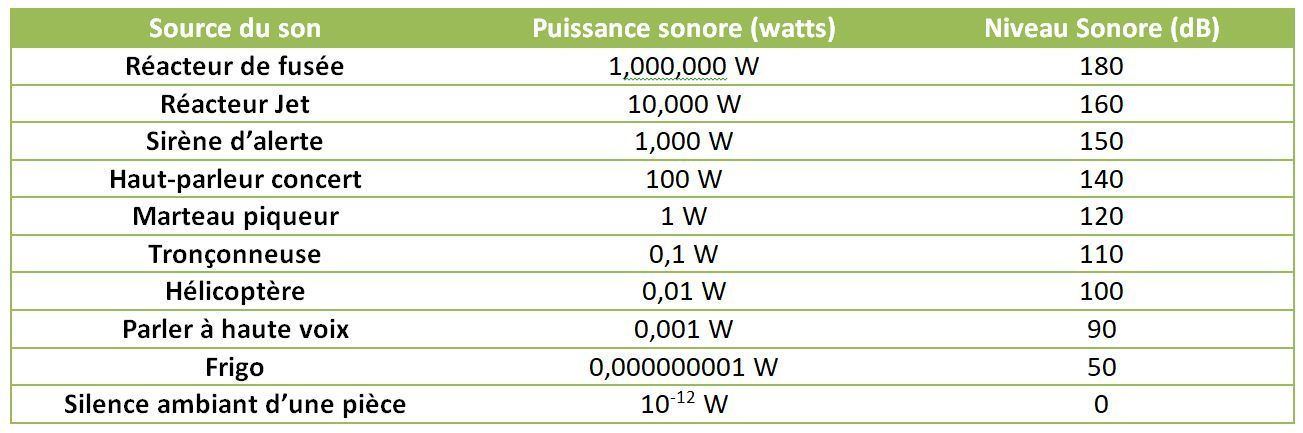
\includegraphics[width=\linewidth]{imgs/p5/puissancesonore.jpg}
    \caption{Quelques puissances sonores}
    \label{fig:puissances}
\end{figure}
\subsection{Intensité sonore}

L’intensité sonore (ou acoustique) est la puissance transportée par les ondes sonores dans une direction donnée, par unité de surface perpendiculairement à cette direction. Elle s’exprime en $W\cdot m^{-2}$. Elle est donnée par la relation : 
\[ I = \dfrac{P}{A}\quad où \quad
\begin{cases}
    P \rightarrow \text{Puissance sonore en }(W) \\
    A \rightarrow \text{aire de la surface recevant le son }(m^2) \\ 
\end{cases}
\]
\begingroup
\begin{wrapfigure}{r}{0.4\textwidth}
  \centering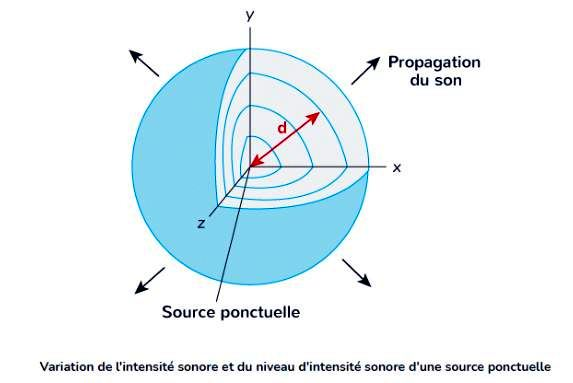
\includegraphics[width=\linewidth]{imgs/p5/sonSphere.jpg}
\end{wrapfigure}

L’intensité sonore diminue en s’éloignant de la source, \textbf{inversement proportionnelle au carré de la distance}. Ceci, comme toute loi en carré inverse, est une sorte de ‘dilution’ de la puissance émise par la source. Au fur et à mesure que l’onde s’éloigne de la source, cette puissance se répartit sur une aire croissante. Ainsi, quand la distance double, cette surface quadruple, et donc, l’intensité se divise par quatre. 

\endgroup
\vspace{1cm}
\subsection{Niveau sonore}
\begingroup
\begin{wrapfigure}{R}{0.35\textwidth}
  \centering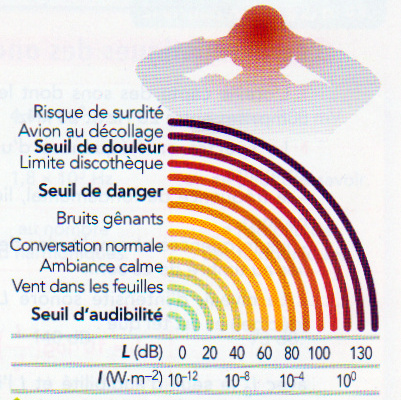
\includegraphics[width=\linewidth]{imgs/p5/niveausonore.jpg}
\end{wrapfigure}

Le niveau sonore est une mesure logarithmique qui définit le niveau d’une intensité sonore en la comparant à une valeur de référence, ici seuil d’audition $I_0=1,0\es{-12}\; W\cdot m^{-2}$. Le niveau sonore $L$ est donnée par la relations : 
\[L_1 = 10\log\dfrac{I_1}{I_0}   \quad où \quad
\begin{cases}
   I_1 \rightarrow \text{Intensité sonore mesurée }(W\cdot m^{-2}) \\
   I_0 \rightarrow \text{Seuil d'audition humaine }(W\cdot m^{-2}) \\ 
\end{cases}
\]

Le niveau sonore s’exprime en \textbf{décibel} ($dB$).

\endgroup
\vspace{1.5cm}
\begin{exo}
Déterminer par quel facteur augmente le niveau sonore, quand on double l'intensité sonore, à une distance donnée. 
\vspace{4cm}
\end{exo}

\begin{exo}
Déterminer de quelle distance il faut s'éloigner d'une source ponctuelle sonore pour que le niveau sonore baisse de $6\;dB$. 
\vspace{4cm}
\end{exo}

\section{Interférences}

\subsection{Phase \& Déphasage}
\begin{itemize}
    \item La phase est une indication de la situation instantanée d’une onde
    \item Le déphasage (ou différence de phase)\eng{Phase angle} entre deux ondes est la différence entre leurs phases. 
    \item Nous représentons le déphasage entre deux ondes de même fréquence, de différentes manières :
    \begin{itemize}
        \item \textbf{Angle $\Delta \varphi$ :} soit $\Delta t$ le décalage temporel en un point quelconque entre deux ondes de même fréquence, et $T$ la période des ondes :
        \[  \Delta \varphi = 2\pi\dfrac{\Delta t}{T}  \quad\quad où \quad\quad  
            \begin{cases}
            \rightarrow t, T\text{ en }(s) \\
            \rightarrow \Delta \varphi\text{ en }(rad) \\ 
             \end{cases}
        \]
        \item \textbf{Temps :  }en comparant le retard temporel d’une onde par rapport à l’autre
        \item \textbf{Distance : }en comparant le retard spatial d’une onde par rapport à une autre.
    \end{itemize}
    \item Si $\Delta \varphi = 2k\pi \; ; \; k\in \mathbb{Z}$; alors les signaux sont \textbf{en phase} 
    \item Si $\Delta \varphi = 2(k+1)\pi \; ; \; k\in \mathbb{Z}$ ; alors les signaux sont \textbf{en opposition de phase} 
\end{itemize}

\begin{wrapfigure}{r}{0.4\textwidth}
  \centering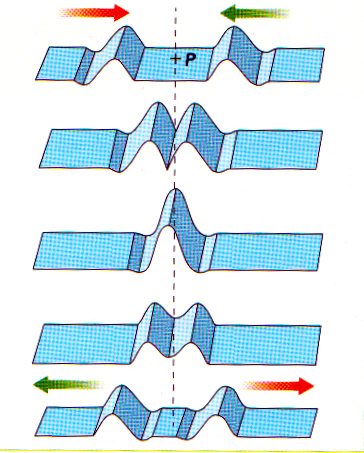
\includegraphics[width=\linewidth]{imgs/p5/interfere.jpg}
\end{wrapfigure}

\begin{defn}{Interférence}
\begin{itemize}
    \item Il y a de l’interférence lorsque deux ondes se croisent, et se \textbf{superposent}.
    \item L’interférence entraîne la création d’une nouvelle onde dont l’amplitude à chaque point de l’espace est la \textbf{somme des amplitudes des ondes en interférence} au point donné. 
        \[ A'= A_1 + A_2 \]
    \item Si $A_1$  et $A_2$  sont de même signe, alors $|A'| > A_1  \text{ ou } A_2$  et on parle d’\textbf{interférence constructive}. Si l’interférence est constructive en tout point, les ondes sont \textbf{en phase}. 
    \item Si $A_1$  et $A_2$  ne sont pas de même signe, alors $A_2<|A'|<A_1$   ou $A_1<|A'|<A_2$ et on parle d’\textbf{interférence destructive}. Si l’interférence est destructive en tout point, les ondes sont \textbf{en opposition de phase}. 
\end{itemize}
\end{defn}
Le phénomène d'interférence est un plutôt singulier, et quelques que l'on ne voit jamais quand il y a du mouvement ET du transport de matière. 

\begin{figure}[ht]
\centering
\begin{subfigure}{.47\textwidth}
  \centering
  % include first image
  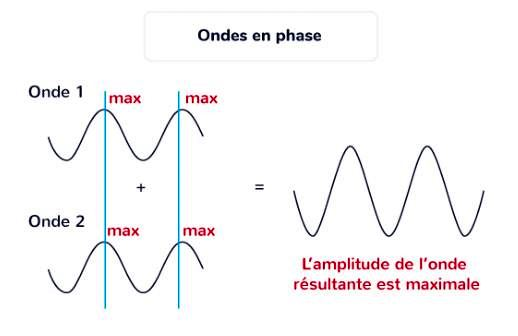
\includegraphics[width=.95\linewidth]{imgs/p5/enPhase.jpg}  
\end{subfigure}
\begin{subfigure}{.47\textwidth}
  \centering
  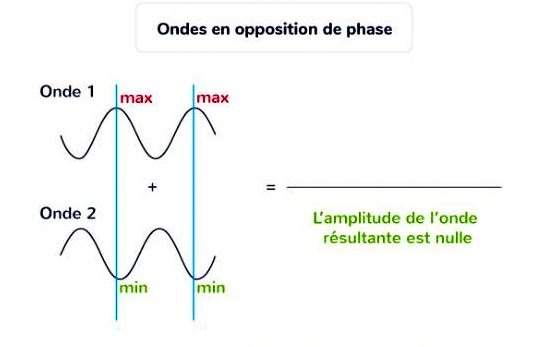
\includegraphics[width=.95\linewidth]{imgs/p5/oppoPhase.jpg}  
\end{subfigure}
\caption{Interférences constructives et destructives}
\end{figure}

\subsection{Experience de Young}

L'expérience de Thomas Young \eng{Young's double-slit experiment} une expérience célèbre qui consiste à faire interférer deux faisceaux de lumière \textbf{issus d'une même source}, en les faisant passer par deux petits trous percés dans un plan opaque. Cette expérience a été réalisée pour la première fois par Thomas Young en 1801 et a permis de comprendre le comportement et la nature de la lumière. Sur un écran disposé en face des fentes de Young, on observe un motif d’interférence \eng{interference pattern} qui est une zone où s'alternent des franges sombres et illuminées.

\begin{figure}[h]
    \centering
    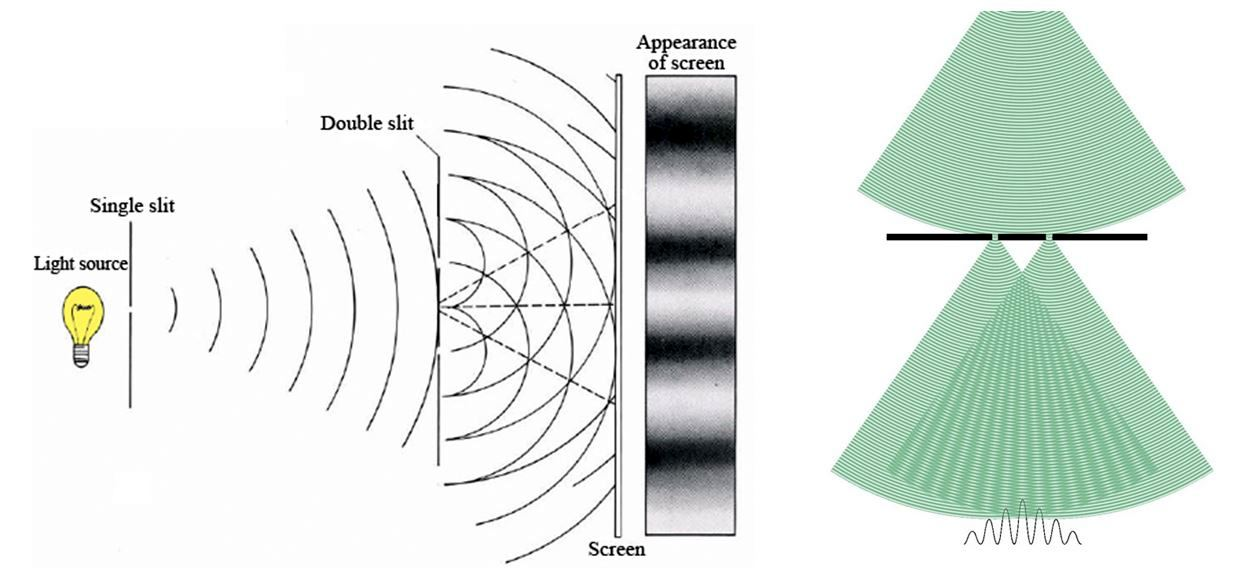
\includegraphics[width=\linewidth]{imgs/p5/young2.jpg}
    \caption{L'expérience double-fentre de Young.}
\end{figure}

\begin{exo} Quelle est donc la signification de cette expérience?  
\vspace{2cm}
\end{exo}

Lors de l’interférence lumineuse, nous voyons des « franges d’interférence ».  En appuyant sur les notions d’interférences constructive et destructive nous pouvons dire maintenant que les franges claires (où l’intensité est maximale) sont dues à de l’interférence constructive ; et là où on trouve des franges sombres il y a de l’interférence destructive.  

La distance séparant deux franges claire/sombre successives, dans le cas des fentes de Young, est :
\[  i = \dfrac{\lambda d}{a}
\quad \quad  où \quad  \quad 
\begin{cases}
    i \rightarrow \text{la distance interfrange } \\
    \lambda \rightarrow \text{longueur d'onde} \\ 
    d \rightarrow \text{distance source-écran} \\
    a  \rightarrow \text{distance séparant les deux fentes} \\
\end{cases}
\]

Le cas d’interférence de la lumière blanche est un peu plus compliqué, car c’est une lumière polychrome, et est donc composée de différentes longueurs d’ondes, correspondant aux différentes couleurs. Dans ce cas-là, l’interférence peut être constructive à certains endroits, et destructive ailleurs. La lumière résultante présente des couleurs interférentielles. C’est en effet le cas de l’\textbf{interférence par une couche mince}\eng{thin-film interference}, comme dans les figures ci-dessous :

\begin{figure}[H]
    \centering
    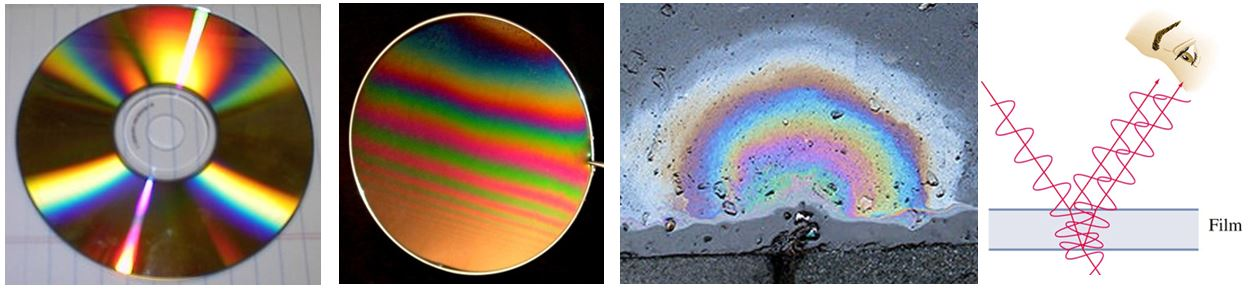
\includegraphics[width=\linewidth]{imgs/p5/thinfilm.jpg}
    \caption{Exemples d'interférence couche mince.}
\end{figure}

\section{Diffraction}

\begin{defn}{Diffraction}
\begin{itemize}
    \item C’est la modification d’une onde progressive lorsqu’elle rencontre un obstacle opaque (i.e. non-transparent), ou un trou sur son chemin. 
    \item Ce phénomène pourrait être interprété comme la diffusion de l’onde par tous les points de l’obstacle. 
    \item Nous observons la diffraction avec de divers phénomènes ondulatoires : lumière, son, vagues, et même avec des particules élémentaires
    \item L’importance du phénomène dépend du rapport entre la longueur de l’obstacle (ou ouverture) et la longueur d’onde de l’onde incidente. Le demi-angle de diffraction $\theta$ est donné par
    \[        
    \theta = \dfrac{\lambda}{a} \quad \quad  où \quad  \quad 
    \begin{cases}
    \lambda \rightarrow \text{longueur d'onde }(m) \\
    a  \rightarrow \text{largeur de l'obstacle/ouverture  }(m) \\ 
    \theta \rightarrow \text{demi-angle de diffraction }(rad)\\
    \end{cases}
    \]
    \item On voit donc que pour que le phénomène de diffraction soit notable, il faut que la largeur a soit du même ordre de grandeur que la longueur d’onde $\lambda$ , ou que $a<\lambda$.  Si $a>>\lambda$ le phénomène de diffraction est négligeable ou inexistant.  
\end{itemize}
\end{defn}
\begin{figure}[H]
\centering
\begin{subfigure}{.27\textwidth}
  \centering
  % include first image
  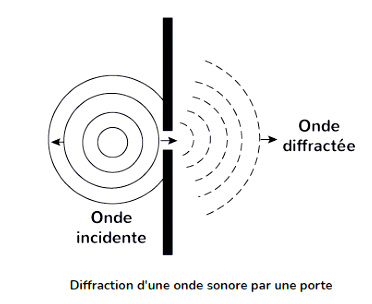
\includegraphics[width=.95\linewidth]{imgs/p5/diffraction.png.jpg}  
\end{subfigure}
\begin{subfigure}{.7\textwidth}
  \centering
  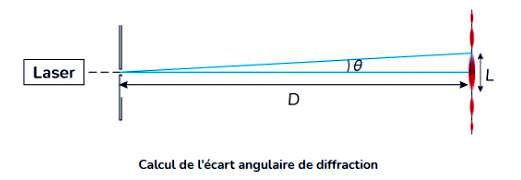
\includegraphics[width=.95\linewidth]{imgs/p5/montageDiff.jpg}  
\end{subfigure}
\end{figure}

\begin{figure}[H]
    \centering
    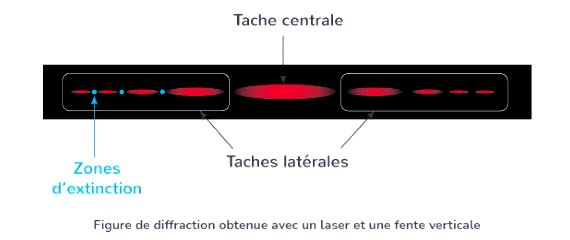
\includegraphics[width=0.9\linewidth]{imgs/p5/motifDiff2.jpg}
\end{figure}
\begin{exo} Quelle est l’ouverture angulaire en degré d’une onde acoustique de fréquence $\nu=4,0\, kHz$ ayant traversé une ouverture de largeur $a=80\, cm$, la célérité étant $c_{onde}=340\, \mps$?
\vspace{3.5cm}
\end{exo}
Il est intéressant de comparer les figures de diffraction et de l'interférence afin de mieux comprendre leurs formes. En effet, le motif d'interférence est le résultats de deux diffractions (des deux fentes) superposés et donc en interférence constructive/destructive, à l'intérieur des tâches de diffraction. 

\begin{figure}[H]
    \centering
    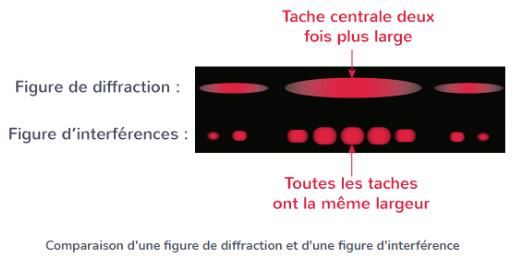
\includegraphics[width=.9\linewidth]{imgs/p5/interfereDIFF.jpg}
\end{figure}
\newpage
\section{Effet Doppler}

Cet effet se manifeste lorsque la source émettrice est en mouvement par rapport au capteur (observateur).  Le signal capté présente une fréquence qui diffère de la fréquence du signal émis. 

\begin{figure}[H]
    \centering
    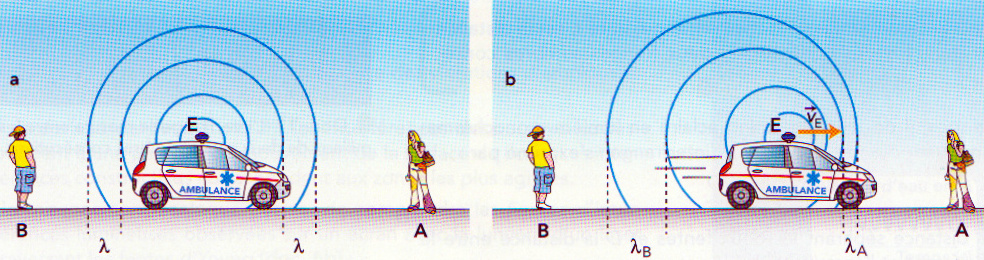
\includegraphics[width=\linewidth]{imgs/p5/doppler.jpg}
\end{figure}

Nous pouvons d’abord expliquer ce phénomène en utilisant une analogie : 

\begin{quote}
   Une personne est debout dans l’eau, au bord du rivage. Des vagues lui arrivent sur les pieds toutes les dix secondes. La personne marche, puis court en direction du large : elle va à la rencontre des vagues, celles-ci l’atteignent avec une fréquence plus élevée (par exemple toutes les huit secondes, puis toutes les cinq secondes). La personne fait alors demi-tour et marche puis court en direction de la plage ; les vagues l’atteignent avec une fréquence moins élevée, par exemple toutes les douze, puis quinze secondes.
   
   La fréquence des vagues ne dépend pas du mouvement de la personne par rapport à l’eau (elle est notamment indépendante de la présence ou non d’un courant), mais du mouvement de la personne par rapport à l’émetteur des vagues (en l’occurrence un lieu au large où le courant s’oppose au vent).    (-wikipédia)
\end{quote}

Nous voulons trouver une relation mathématique établissant un lien entre la variation de la fréquence perçue, et la vitesse relative de la source du son par rapport à l'auditeur. 

\begin{itemize}
    \item Considérons une source en mouvement avec une vitesse de $v_e$  émettant régulièrement des « bips » avec une période de $T_e=\nicefrac{1}{f_e}$. 
    
    Supposons que le capteur se situe à une distance $d_0$  de la source à la date $t=0$, et finalement que l’onde sonore se propage avec une célérité de $c$.
    \item Le temps à mettre pour que l’onde parcoure cette distance est : $t_1=\nicefrac{d_0}{c}$. Donc le capteur reçoit le premier « bip » à l’instant $t_1$.

\begin{figure}[H]
\centering
\begin{subfigure}{.47\textwidth}
  \centering
  % include first image
  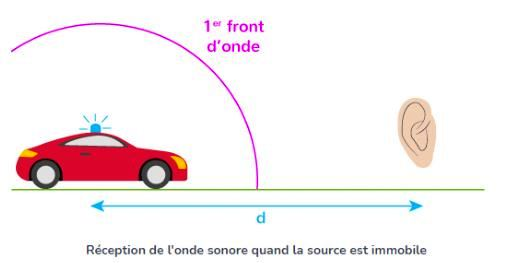
\includegraphics[width=.95\linewidth]{imgs/p5/dop1.jpg}  
\end{subfigure}
\begin{subfigure}{.47\textwidth}
  \centering
  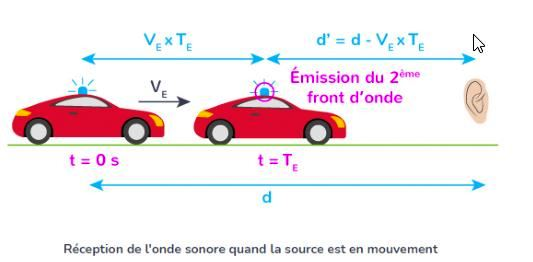
\includegraphics[width=.95\linewidth]{imgs/p5/dop2.jpg}  
\end{subfigure}
\end{figure}

    \item L’émetteur envoie un deuxième « bip » à l’instant $t=T_e$. L’émetteur s’est déplacé entre temps, et la distance émetteur-capteur est maintenant 
    \[ d_0' = d_0 -v_eT_e = ct_1 - v_eT_e \]
    \item Le capteur reçoit le deuxième « bip » à 
    \[t_2 = \dfrac{d_0'}{c} + T_e = \dfrac{ct_1 - v_eT_e}{c} + T_e \]
    \item Pour le capteur, la durée $T_A$  entre deux « bips » est
    \begin{align*}
    T_A &= t_2 - t_1 \\
        &= \dfrac{d_0'}{c} + T_e - \dfrac{d_0}{c} \\
        &= \dfrac{1}{c}\left(d_0 - v_eT_e\right) + T_e - \dfrac{d_0}{c} \\
        &= T_e - \dfrac{v_eT_e}{c} \\
        &= T_e \left(1 - \dfrac{v_e}{c}\right) \\
    \end{align*}
    \item Pour le capteur donc, la période est : 
    \[ T_A = T_e \left(1 - \dfrac{v_e}{c}\right) \]
    \item et la fréquence : 
    \[ f_A = f_e\left( \dfrac{c}{c - v_e}\right) \]
\end{itemize}
 
Nous avons donc montré que si la source est en mouvement par rapport au capteur, le capteur n’observera pas la fréquence émise du signal, mais une autre fréquence qui dépend de la vitesse relative entre la source et le capteur. 

\begin{exo}
Déterminer l'expression de l'effet Doppler dans le cas où la source s'éloigne du récepteur. 
\vspace{4cm}
\end{exo}
\begin{rmrq}
La relation que nous avons trouvée est seulement \textit{une} relation possible, étant donné la relativité d'un mouvement. En effet, l'effet Doppler est aussi valable dans le cas ou la source est immobile avec un récepteur en mouvement, ou dans le cas le plus général possible avec la source et le capteur en mouvement à la fois. 
\end{rmrq}

\begin{exo}
On utilise des ondes ultrasons pour déterminer la vitesse d'un objet qui nous rapproche. Le décalage de doppler est de $\delta f = 50\; Hz$. Déterminer sa vitesse. 
\vspace{4cm}

\end{exo}


\subsection{Applications de l'Effet Doppler}

\subsubsection{Astronomie}
L’effet Doppler est particulièrement précieux en astronomie car il renseigne à la fois sur le mouvement des astres et sur les mouvements de matière à l’intérieur de ces astres.

L’effet Doppler permet de déterminer directement la vitesse radiale d’une étoile. En effet, en étudiant le spectre d’un astre, on constate que les raies spectrales sont décalées en longueur d’onde par rapport aux mêmes raies observées en laboratoire. Le décalage d’une raie visible se produit soit vers le rouge \eng{Red Shift}, ce qui indique que l’étoile s’éloigne, soit vers le bleu\eng{blue shift}, si elle se rapproche.

La mesure de la vitesse des étoiles ou des nuages de gaz interstellaire a permis de préciser les mouvements de matière à l’intérieur de la Voie lactée et d’en déterminer la structure spirale.
\begin{quote}
  La loi de Hubble tire son nom de l'astronome américain Edwin Hubble qui la publia en 1929. Elle fut la première preuve de l'expansion de l'univers, un phénomène générique prédit par la relativité générale, et du Big Bang, le modèle cosmologique qui en résulte le plus naturellement. Hubble découvrit cette loi en observant un décalage vers le rouge  (i.e. manifestation de l’effet doppler pour les ondes lumineuse presque systématique dans les galaxies dont il avait découvert auparavant la nature exacte à l'aide de l'observation d'un certain type d'étoiles variables, les céphéides. Ces étoiles sont sujettes à des variations de luminosité dont la période est reliée à la luminosité absolue suivant une loi établie par l'astronome Henrietta Leavitt au début du XXe siècle. L'observation de la période de variation des céphéides dans une autre galaxie permettait ainsi de déduire leur distance relative. La vitesse de fuite de ces mêmes galaxies était, elle, mesurée par l'observation d'un décalage vers le rouge de leur spectre, effet interprété comme étant dû à leur mouvement de fuite.   (-wikipédia)  
\end{quote}

\subsubsection{Radar}
Un radar est un appareil qui émet des paquets d’ondes et écoute ensuite le retour de cible. Si ces cibles se déplacent, un effet Doppler est engendré ce qui permet d’en tirer la vitesse radiale de leur déplacement. Le radar peut donc être adapté pour utiliser ce principe.
\begin{itemize}
    \item Radar de contrôle routier : la police et la gendarmerie utilisent des radars pour déterminer la vitesse des automobiles. Pour cela ils utilisent un radar dont la fréquence est parfaitement connue. La mesure de la fréquence de l’écho donne la vitesse du véhicule. La technologie moderne permet aujourd’hui d’avoir des radars automatiques et des jumelles-laser.
	\item Radar de mesure balistique : de nombreuses mesures balistiques sont effectuées grâce au radar Doppler. Il permet de mesurer la vitesse du projectile (calibre de $1\; mm$, éclat par exemple jusqu’au missile), et surtout la mesure du $v_0$ (vitesse initiale du projectile à la sortie de la bouche du canon), de la vitesse à l’impact (mise au point de gilet pare-balle, par exemple), de la vitesse de rotation du projectile, ainsi que de sa trajectographie et de son coefficient de traînée. 
\end{itemize}
	
\subsubsection{Médecine}
\begin{itemize}
    \item Le doppler, couplé ou non à un examen échographique, permet d’analyser la vitesse du sang. On peut ainsi quantifier des débits, des fuites ou des rétrécissements.
    \item En effet, l’échodoppler est utilisé en médecine pour mesurer la vitesse des hématies et pour calculer le diamètre d’un vaisseau sanguin (aorte…).
	En cardiologie, on peut analyser la vitesse des parois cardiaques à l’aide du doppler tissulaire, c’est l’imagerie doppler des tissus, ou TDI (tissul doppler imaging)
\end{itemize}

\section{Exercices Résolus}	
\begin{figure}[H]
    \centering
    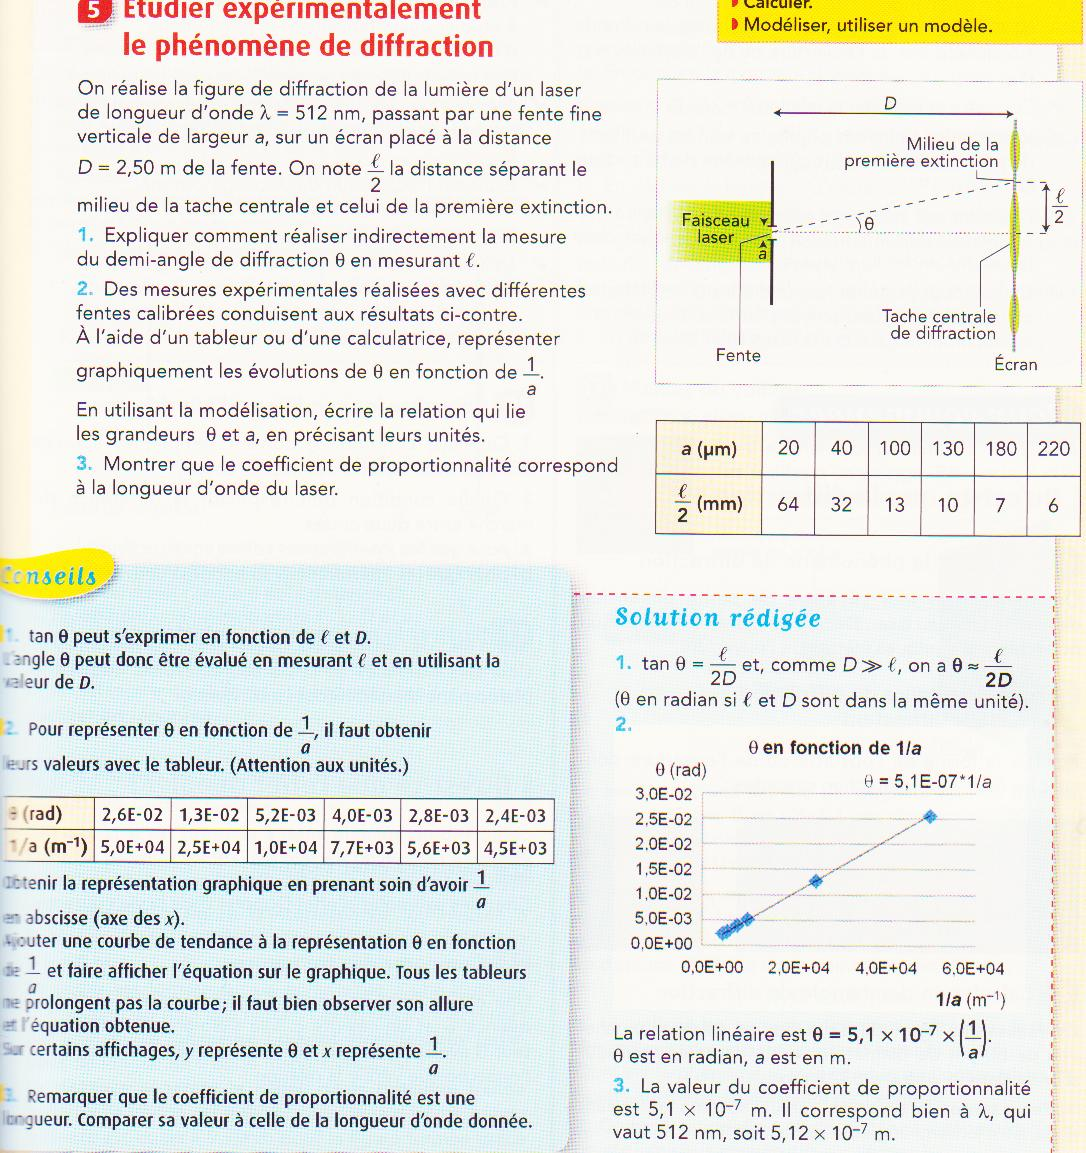
\includegraphics[width=\linewidth]{imgs/p5/exoDIFF.jpg}
\end{figure}
\begin{figure}[H]
    \centering
    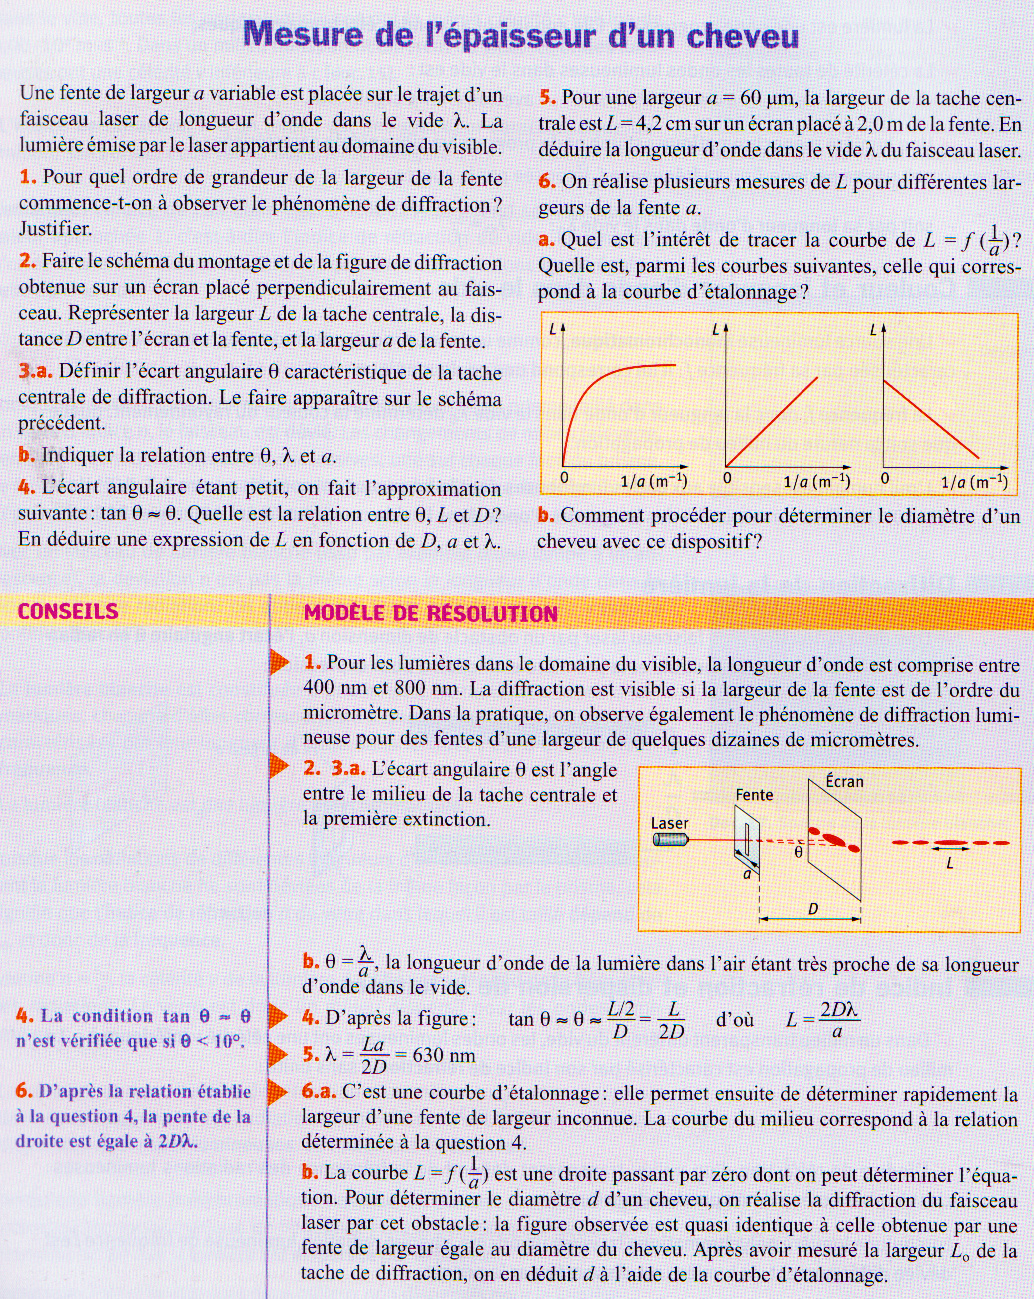
\includegraphics[width=\linewidth]{imgs/p5/exoCHEVEU.jpg}
\end{figure}
\begin{figure}[H]
    \centering
    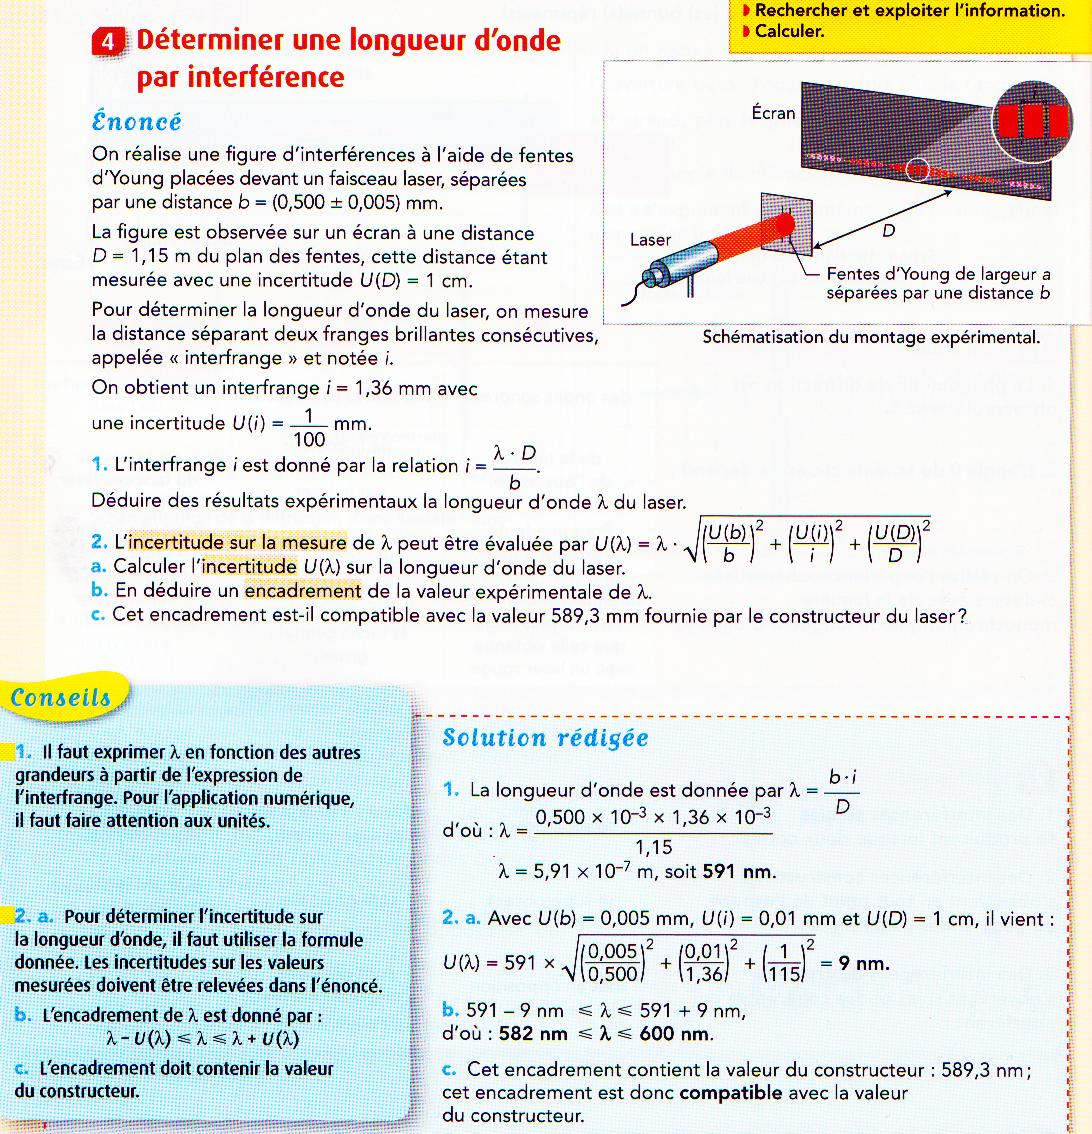
\includegraphics[width=\linewidth]{imgs/p5/xoINTERFER.jpg}
\end{figure}

\end{document}